\documentclass[thesis, a4paper, 11pt]{Format}
\usepackage{CJKutf8} % Chinese language support.
\usepackage{textcomp} % For registered symbol.
\usepackage{booktabs} % Generate tables.
\usepackage{listings} % List code.
\usepackage{color} % Code highlight colors.

\definecolor{Numbers}{rgb}{0.5, 0.0, 0.0}
\definecolor{Strings}{rgb}{0.0, 0.65, 0.0}
\definecolor{Keywords}{rgb}{0.0, 0.0, 1.0}
\definecolor{Comments}{rgb}{0.0, 0.65, 1.0}
\definecolor{Background}{rgb}{0.9, 0.9, 0.9}

\lstset{ 
	backgroundcolor=\color{Background},
	commentstyle=\color{Comments},
	keywordstyle=\color{Keywords},
	numberstyle=\tiny\color{Numbers},
	stringstyle=\color{Strings},
	basicstyle=\ttfamily\small\setstretch{1},
	captionpos=b, % Set the caption-position to bottom.
	frame=single, % Add a frame around the code.
	numbers=left, % Line-numbers are on the left hand side.
	numbersep=5pt, % The distance between line-numbers and the code.
	stepnumber=1, % Each line will be numbered.
	tabsize=4,
}

\renewcommand{\baselinestretch}{1.5}
\makeindex

\graphicspath{{Figures/}} % Specify paths where figures are located.

\begin{document}
	\pagenumbering{alph} % This is needed to clear certain issues with the hyperref package.

	\addToPDFBookmarks{0}{Front}{rootNode}
	% Create a root node named "Front" in the pdf bookmarks.

	\pagenumbering{roman}
	\addToPDFBookmarks{1}{Title}{i}
	\makeTitlePage

	\addToPDFBookmarks{1}{Abstract}{ii}
	\chapter*{Abstract}\label{ch:abstract}
In this project, we concentrated on recognising oracle bone script characters, an ancient Chinese writing system and basis of modern Chinese characters, by applying the latest deep learning approaches; also a GAN-based data augmentation method was used to convert pre-existing oracle bone scripts into bronzeware-similar characters. All files and data set mentioned below in this thesis can be accessed in our project GitHub repository: \url{https://github.com/Ancient-Discovery/Colosseum}, licensed under the Mozilla Public License 2.0.

	\addToPDFBookmarks{1}{Acknowledgements}{iii}
	\chapter*{Acknowledgements}
Firstly, I would like to appreciate my supervisor Dr. Ruihai Dong for bringing me into deep learning domain, a fast-growing AI field with huge opportunities. During the whole semester, his continuous support made me accomplish the entire research project.

Secondly, I really thank UCD school of Computer Science for partially covering fares of our team on-the-spot field study in Anyang, Henan Province, from April 4 to 5, 2018. Also, I want to express huge thank to my uncle Yanjun Ren who introduced us plenty of local connection, which provided a few academic help from them.

Eventually, I finalise my acknowledgements by appreciating highly efficient collaboration with my other team members for nearly four months, Lin Lyu and LuLu Wang; especially my ex-girlfriend Lin, who supported me a lot previously and made the break-up much less nasty.

	\addToPDFBookmarks{0}{Table of Contents}{iv}
	\tableofcontents

	%\addToTOC{List of Tables}
	%\listoftables
	\addToTOC{List of Figures}
	\listoffigures

	\newpage
	\pagenumbering{arabic}
	\setcounter{page}{1}

	\chapter{Introduction}\label{ch:introduction}
Oracle bone script is one of the earliest known Chinese writing systems, dating back to around 3000 years ago, which were engraved on animal scapulae or turtle plastrons (flat under-part of shells) with sharp stones or bronze instruments. Since the first piece of oracle bone scripts was found and catalogued by scholars in Anyang, the primary capital of the late Shang Dynasty, which ensured undoubtedly the authenticity of existence of pre-Zhou-Dynasty history, hundreds of thousands of bone fragments were dug along with numerous artefacts on site in subsequent archaeological excavations. They contain more than 30000 distinct symbols, estimated to be variant forms of around 4600 identified individual characters; these new materials are of importance for Chinese palaeography and research into prehistoric civilisation. Majority of oracle bones at that time was associated with pyromancy (divination by fire), by inscribing questions on shoulder blades, burning them and interpreting occurring cracks formed on the surface as divine responses, which were engraved on the polished surface alongside the cracks. And analysis indicates that most of text constitutes hunting expeditions, weather, warfare, astronomical events, administrative orders and selection of auspicious for important ceremonies\cite[pp.~5]{de2000sources}. Oracle bone scripts are almost identical with modern functional writing system in use currently; highly advanced and surprisingly mature, oracle bone scripts achieve a very high extent of abstraction in terms of expressing meanings. A whole scientific discipline called Oracle Bone Studies was set up, dedicating to deciphering them and reconstructing lives of Shang residents or confirming succession of kings. Compared to bronze scripts later on, preceding oracle bone scripts appear to be of raw simplicity, obviously because the difficulty of engraving symbols on materials with firm surface could not be overcome easily at that time.

However, just 1300 ones can be translated to their modern counterparts by linguists. Occasionally many recognised characters are still disputed due to lack of definitive explanations. Structures and orientations of each character varied largely in different time periods, which sets an even higher barrier for researchers. Deciphering one new symbol could reveal plenty of new facts in the ancient society.

And machine learning, a main sub-field of artificial intelligence, revived increasingly in recent years after nearly twenty years of AI winter due to tremendous hardware performance increase; it involves statistical techniques to improve performance of specific problems by feeding data instead of being explicitly programmed and its applications covers all industrial domains. After AlphaGo, a computer program developed by Google Deepmind, beat 9-dan player Lee Sedol without handicaps in March 2016, deep learning, one of classical machine learning algorithms inspired by biological nervous systems, gradually became well-known by public. The most major difference between deep learning and traditional machine learning is the scale of data. The more amount of data a program is fed in, the better results deep learning will achieve typically. As opposed to task-specific algorithms, models generated by deep learning can be transferred to various types of problems without completely rewriting code. And with assistance of deep learning, character recognition, a field of research in pattern matching, computer vision, and certainly artificial intelligence itself, has developed rapidly. And recognition based on image processing (correlation) and feature detection easily makes a breakthrough and avoids bottleneck even with high-end hardware.

In this project, we merged two separate disciplines together, via applying several latest deep learning techniques to speed up the process of recognising oracle bone script characters, which can be an potential academic helper for Chinese palaeography. And then we applied supervised deep learning, with both paired and unpaired data, to create two types of GANs, generative adversarial networks, in order to generate bronze inscription images from oracle bone script patterns or vice versa.
	\chapter{Literature Review}
The literature review is aggregated with three sections, covering topics Chinese character recognition \& generation, neural networks and mathematical morphology respectively, which are highly connected with our project as background technical information.

\section{Chinese Character Recognition \& Generation}
When it comes to automatic recognition or generation of actual oracle bone scripts, there are very limited resources. Most of them still work on establishment of fundamental computer tools for research, Shi et al.\cite{Shi2005} digitalised scanning photos of oracle bone scripts, turning them into vector graphs in .svg format for web use; Liu et al.\cite{Liu2004} wrote a Visual C++ application on Windows as visual input method for oracle bone script characters. And when we turned ourselves to modern Chinese character recognition and hope that such researches can guide us to a correct track, a lot of relative papers were found. Previous work on Chinese character recognition based on neural networks was mainly in handwritten character, which was considered as a difficult task generally. In 2010, Chinese handwriting recognition contest\cite{5659229} showed that for GB2312-80 level-1 set, the most frequently-used modern Chinese character set in mainland China, off-line recognition accuracy of the top system (HKU) reached only 89.99\%, let alone oracle bone scripts which has no standard uniform glyphs decided by academia.

Based on these facts, Xue et al.\cite{xue2014recognition} decided to improve accuracy by distinguish between easily confused Chinese characters; authors combined character feature extraction and feature dimension reduction together, providing a new CNN-based similar character recognition system. Xu et al.\cite{xu2008automatic} proposed a method which trains machine to learn calligraphic handwriting style of a specific writer. And Xu et al.\cite{1439477} also invented an algorithm that enables the computer to generate Chinese calligraphic handwritings with special aesthetic requirements learnt from training samples.

In \cite{7327196}, authors collected a dataset called Oracle-20K from Chinese Etymology\footnote{\url{http://hanziyuan.net}, which is also one of our data sources.}, a data set of sketching objects distributed over 250 different categories, and claimed that their dataset was the largest oracle character dataset in computer vision so far, although they did not actually release it. To build the dataset, they removed all glyphs which contain less than 25 unique samples and eleven low-level representations in total and four mid-levels ones (based on multi-layer sparse autoencoder) were used to represent oracle bone scripts.

Eventually, Liu et al.\cite{6376394} introduced a unique approach to generate personal handwriting style for Chinese characters, which is quite close to what we planned to do. First a Chinese character is split into parts represented quantitatively by multi-dimensional vectors, ``such as strokes, radicals and frequent character components''. After analysing on topological structure of the whole character and spatial relationships between each component, authors put forward a representation ``parameterising the character's topological structure, its layout, as well as the relative length distribution of two strokes''. And later on an overall similarity between two components can be calculated, used in handwriting facsimile.

\section{Neural Networks}
Neural network, also referred as artificial neural network, a computational model which is a vaguely simplified version of biological neural networks, consisting of animal brains. Neural networks constitutes a set of connected nodes called neurons, a mathematical function that sums up all weighed inputs (signals) from other neurons and applies an activation function on it as outputs. And activation functions used in neurons are often non-linear like logistic functions, or rectified linear (ReLU) function. And connections are referred as edges in neural network context. The weight changes by back propagation and sometimes neurons may have a threshold to decide if the signal is sent or not. Typically neurons are divided into multiple layers and different layers apply different types of transformations.

\subsection{Convolutional Neural Networks}
Nowadays, convolutional neural network (CNN or ConvNet) is considered as a prevalent model for image classification. This model resembles original neural networks with ``learnable'' weights and biases, applying loss function (like SoftMax function that we used in our project) to last layer. It is a type of multilayer perceptrons with several levels of hidden layers, including convolutional layers, pooling layers and finally, fully connected layers.

CNN can result in high accuracy rates, even better than human performance in some cases like MNIST recognition. Besides, CNN becomes very efficient by using filters. ``CNNs have much fewer connections and parameters and so they are easier to train''\cite{Krizhevsky:2012:ICD:2999134.2999257}, and involves relatively not intensive preprocessing. In CNN, every single neuron represents a small part of the vision of an image (local receptive field), and all neurons cover all the information in a single image.

\subsection{Generative Adversarial Nets}
To elaborate GANs, we have to go through briefly details on generative model and its counterpart discriminative model from mathematics first. In statistics and probability, a generative model is a statistical model about generation of sample or similar data from a larger population and it learns the joint probability distribution $ P(X, Y) $ and given the same arbitrary input $ X $, conditional probability of $ Y $ can be calculated, $ P(Y | X) $, which a discriminative model can learn from. And for instance, in binary classification problems, if output $ Y $ is greater than some pre-set threshold $ Z $, $ X $ belongs to group $ W_1 $; otherwise, $ X $ is in group $ W_2 $.

And the ultimate task of supervised learning is to build a model (classifier) learned from bulks of data. Therefore, generative adversarial nets is proposed by Ian Goodfellow in 2014\cite{goodfellow2014generative} and offers a new method of deep learning representations without plenty of labelled data. Obviously, GAN is not the only way to apply neural networks in unsupervised learning; auto encoder\cite[ch.~14]{Goodfellow-et-al-2016} and Boltzmann machine\cite[ch.~20]{Goodfellow-et-al-2016}. Previously, two of them worked on extracting features from the equation $ f(x) = x $ and train and generate samples relying on Markov chain and approximate inference\cite[ch.~20]{Goodfellow-et-al-2016}, which are really calculation-consuming; GAN copes with this issue and is not limited to several Markov-suitable probability distribution.

GAN derived from two-player game in game theory and two players are generative model $ G $ and discriminative model $ D $ respectively. Model $ G $ captures data distribution, using data whose noise subjects to uniform / normal distribution to a generate similar real training sample. For this sample itself, it should try it utmost to resemble the real one. In the meantime, discriminative model $ D $ is a binary classifier (which returns probability values) that judges if a sample comes from the training set rather than $ G $. During the whole training process, one side is fixed and the other's network weight is keeping updating and vice versa. Via back propagation, two networks update separately and ``compete'' each other, by optimising their networks simultaneously until reaching Nash equilibrium. At that time, generative model $ G $ subjects to distribution of training data, which indicates that it generates identical data. And discriminative model $ D $ cannot distinguish at all, whose accuracy is around 50\%.
\begin{figure}[h]
	\centering
	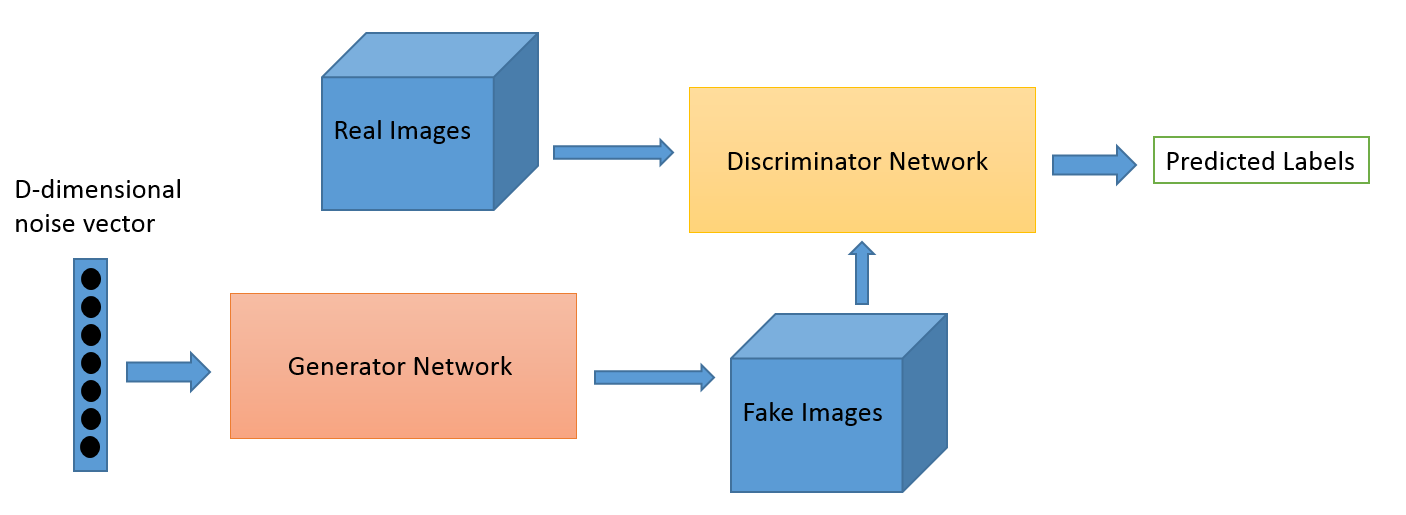
\includegraphics[width=\linewidth]{GAN_Schema.png}
	\caption{General GAN structure (Credit: O'Reilly)}
\end{figure}
And the whole process can be summarised in mathematical fashion as a minimax two-player game:
\[ \underset{G}{\min}\,{\underset{D}{\max}\,V(D, G)={\mathbb{E}_{x\sim{p_{data}(x)}}[\log{D(x)}]+\mathbb{E}_{z\sim{p_{z}(z)}}[\log{(1-D(G(z)))}]}} \]

And this seem-to-be-simple model is vital in the whole history of machine learning. While massive data is available, such as images, voice recordings or plain texts, generative models help us simulate the distribution of these high-dimensional data, which is very futile in many applications. On the other hand, for situation where data is difficult to collect, generative models can create a huge amount of high-quality data and improve efficiency of semi-supervised learning; basically, the whole field of data augmentation is based on it. Specifically, adversarial training can change how we teach AI to fulfil complicated tasks. And in some aspects, these programs learn to become human experts in such a domain.

Although GANs offer us a novel insight into dealing with complex problems, which introduces game theory into machine learning and has extensive impacts, it still has plenty of issues needed to be solved. First and foremost, at least in image generation field, it is not easy to tell how much better GAN is compared to other image generation methods like variational auto-encoder (VAE) or Bayesian networks. It is even harder to prove which one is more efficient: GAN or its derived algorithms. Pitifully, there is not an objective well-accepted standard to gauge difference of various image generation methods; it is inevitably difficult even for human since we judge the genuineness of one image from a few aspects including clearness, object edge colour and appearance of anti-intuitive objects. Only with a reasonable measure method, GAN can be improved systematically.

In GAN, the pictures mapped from the input images to output images domain may have a lot of possibilities which all satisfy the distribution of the output images domain and collapse problem exists. Therefore, researchers\cite{DBLP:journals/corr/ZhuPIE17} proposed CycleGAN (Cycle-Consistent Adversarial Networks) which solved this problem by adding a reverse mapping cycle to enhance the limitations of the conversion. Besides, 70\% of oracle bone scripts do not have paired recognised characters, while CycleGAN is a solution for unpaired image-to-image translation. However, both concluded that it often successes when changing colour and texture of objects. But the task barely succeeds when it requires geometric change, for example, changing a cat to a dog. This happened because the generator architecture is designed for appearance changes.

And the CGAN (Conditional GAN)\cite{DBLP:journals/corr/MirzaO14} is from famous Stanford Computer Vision Lab and it is the first time to come up an idea that adds limitations on GAN to increase accuracy since images generated from original GAN are largely vague in practice. Although the improvement was considered as ``straightforward'', it was highly effectively:
\[ \underset{G}{\min}\,{\underset{D}{\max}\,V(D, G)={\mathbb{E}_{x\sim{p_{data}(x)}}[\log{D(x \mid y)}]+\mathbb{E}_{z\sim{p_{z}(z)}}[\log{(1-D(G(z \mid y)))}]}} \]
Data are labelled in both generative and discriminative models and according to authors' experiments, new generated images contains far more textures.

And the model structure in Pix2Pix\cite{DBLP:journals/corr/IsolaZZE16} resembles work of CGAN. Pairs of same-size pictures are combined as inputs, which changes from three colour channels (RGB) to six ones (which merges two images together), and also $ D(X) $ is replaced by $ D(X, Y) $. And generator $ G $ first encodes input image $ X $ in vector form and decodes to generate image $ Y $. In order to guarantee the high similarity between output image and target one, L1 loss is introduced and makes generated images sharp to a huge extent. And U-Net, closed to residual network, is also used in the paper to merge convoluional kernels from original images to generated ones and reduce much calculation. Noticeably, Pix2Pix introduced a trick called patch, used in Nvidia HD image generation\cite{DBLP:journals/corr/abs-1711-11585}; all images are fed as inputs in partitioned \textbf{patches} form rather than complete images, wherever in generators or discriminators.

\section{Mathematical Morphology}
According to Oxford English Dictionary, morphology, a word borrowed from biology, originally means a study or research of ``the form and structure of animals and plants''. And mathematical morphology (MM) is a framework for image processing based on lattice theory, random geometry\cite{serra1983image} and set theory and is a useful tool for inspecting geometric structures in images\cite{soille2013morphological}. MM ``tends to simplify image data preserving their essential shape characteristics and eliminating irrelevancies''\cite{haralick1987image}, which is suitable for our case since pixel reduction will dramatically speed up tensor-related operations. In this section, a brief introduction mainly highlights structuring element and four basic operators of MM, which are used as thinning algorithm in our code partly.

When a morphological transformation is applied, two inputs are needed: the original image and the SE which decides the nature of operation. The structuring element (SE) is in essence a pre-defined binary shape or template considered as masks normally in matrix form that goes through the image, modifies the pixels based on its ``surrounding neighbours'' it in different methods, providing a huge range of effects on the whole image. It is ``applied to interact with the image to get the resultant''\cite{ravi2013morphological}. The structuring element is therefore typically smaller than the whole image with odd size, not only in number of pixels (or area in the continuous case), but the pixels are also close to each other. ``Size of the structuring element, acts as a 'window' over which the interaction takes place''\cite{ravi2013morphological}. and they ``slide over the image and transform it''. According to \cite{ravi2013morphological}, the structuring element is ``positioned at all possible locations in the image and it is compared with the corresponding neighbourhood of pixels''. Operations on binary images create a new binary ones.

And let $ E $ be a Euclidean space, and $ A $ and $ B $ are binary images in $ E $. And basic operators in MM are listed as followed:
\begin{itemize}
	\item \textbf{Erosion} A method to remove the pixels of foreground edges; it can be represented as $ A \ominus B = \{z \in E \mid B_z \subseteq A\} = \displaystyle \bigcap_{b \in B}^{}A_{-b} $.
	\item \textbf{Dilation} It is just opposite of erosion and enlarges boundaries of foreground area and formal mathematical notion is $ A\oplus B=\bigcup_{b\in B}^{} A_b $.
	\item \textbf{Opening} A method to remove edges of foreground in a less destructive way and the definition is $ A \circ B = (A \ominus B) \oplus B = \displaystyle \bigcup_{B_x\subseteq A}^{} B_x $.
	\item \textbf{Closing} An opposite method to opening tends to extend image area, which is defined as $ A \circ B = (A \oplus B) \ominus B $.
\end{itemize}
	\chapter{Environment Setup}\label{ch:setup}
Here we introduction our project environment setup, including related software selections and installations.

\section{Hardware Preparation}
Here we use a high-end remote server located in Ireland, by courtesy of University College Dublin, with seventy-two Intel Xeon\textsuperscript{\textregistered} E5-2695 CPUs and four Nvidia GeForce\textsuperscript{\textregistered} GTX 1080 Titan GPUs running on Ubuntu 16.04 LTS (Xenial Xerus).

\section{Python Version Selection}
Both Python 2.x and 3.x are pre-installed for Ubuntu. Here are listed what is considered in terms of selecting between Python 2.x and 3.x: in the world of Python 2, \texttt{str} object has to be converted to a Unicode object right after calling \texttt{str.decode('utf-8')} on the ground that Python 2 interpreter just treats it as a sequence of bytes rather than real Unicode characters. Therefore, for a statement like \texttt{len(unicode\_str)}, the reture value is the size of bytes stored in memory, which may not equal to the number of readable characters on screen (considering that one Unicode character could hold up to 6 bytes in UTF-8 encoding system). In Python 3, however, the largest difference is that the \texttt{str} type actually holds UTF-8 characters in UTF-8, which is a one-off solution to avoid nastiness since we have to cope with Unicode characters all the time.

\section{TensorFlow}
TensorFlow\footnote{\url{https://www.tensorflow.org/}} is an open source (under Apache 2.0 License) deep learning programming framework maintained by Google Brain team, which uses C++ as the development tool for performance, and provides Python and C APIs with automatic differentiation resembling Theano\footnote{\url{http://www.deeplearning.net/software/theano/}}; it uses ``unified dataflow graph to represent both the computation in an algorithm and the state on which the algorithm operates''\cite{DBLP:journals/corr/AbadiBCCDDDGIIK16}, with edges carrying multidimensional data arrays (a.k.a. tensors) and nodes representing actual mathematical operations applied on them. And it allows users to run each node from TensorFlow programs on different architectures (desktop CPUs, GPUs, TPUs and even mobile platforms) flexibility. Originally only for Google Brain Team's internal use, it was released on November 2015, and became a de-facto industrial standard of deep learning. Compared to other framework in this domain, one of obvious disadvantages is lack of support for OpenMP and OpenCL, which is not an issue at all in our case.

And according to \cite{DBLP:journals/corr/BahrampourRSS15}, though TensorFlow performance of running LeNet and AlexNet ``on a single GPU is not as competitive compare to the other studied framework'', compared to Theano, TensorFlow offers the even more flexible multiple GPU support among all popular deep learning libraries, which is the reason that we insists using multiple GPUs to squeeze performance. Therefore, we use TensorFlow for its customisation, flexibility and popularity.

\section{Related software Installation}
To make GPUs fully work on Ubuntu, from our painful experience, we highly recommend one who works on similar specification to install CUDA Toolkit legacy version \texttt{9.0}\footnote{\url{https://docs.nvidia.com/cuda/cuda-installation-guide-linux/}} instead of the newest version 9.1, cuDNN SDK v7\footnote{\url{https://docs.nvidia.com/deeplearning/sdk/cudnn-install/\#installlinux}} and update Nvidia GPU drivers\footnote{\url{http://nvidia.com/driver}} \textbf{before} installing TensorFlow and its virtual environment Virtualenv (if necessary).

Typically, for one computer which installs Python 3.4+, pip\footnote{\url{https://pypi.org/project/pip/}}, a tool for Python package management, is all set and can only run the command below:

\textbf{(with root privilege)} \texttt{pip3 install tensorflow-gpu}

Currently the latest GPU version of TensorFlow is v1.8.0. All installed packages are listed below: \texttt{absl, astor, bleach, gast, grpcio, html5lib, numpy, protobuf, tensorboard, termcolor, werkzeug, tensorflow-gpu}.

In terms of image processing, ImageMagick\textsuperscript{\textregistered}, a free and open source software suite for converting and editing images in console, offer us three useful commands: \texttt{identify} (used to describe the formats and characteristics of one or more image files), \texttt{mogrify} (used to resize an image, blur, crop, despeckle, dither, draw on, flip, join, re-sample and overwrite the original file) and \texttt{convert} (similar to \texttt{mogrify}, used only to do conversion between images). Installing it by:

\textbf{(with root privilege)} \texttt{apt install imagemagick}

\section{Other Python Packages}
There are other Python packages that we used to build our project:
\begin{itemize}
	\item \textbf{Scipy}\footnote{\url{https://www.scipy.org/}} A huge library of scientific computing, built on multidimensional array provided by \texttt{Numpy}; used to apply sparse matrix calculation.
	\item \textbf{Matplotlib}\footnote{\url{https://matplotlib.org/}} A Matlab-like 2D plotting library; used to display data distribution visually.
	\item \textbf{Requests}\footnote{\url{http://docs.python-requests.org/}} An elegant API to send HTTP/1.1 requests rather than built-in Python library \texttt{urllib2}; used in web crawler part of our project.
	\item \textbf{Pillow}\footnote{\url{https://pillow.readthedocs.io/}} A friendly fork of original PIL (Python Imaging Library); a lightweight library to process images; used to load images into tensors.
	\item \textbf{OpenCV}\footnote{\url{https://opencv.org/}} A powerful free image processing library with Python implementation under a BSD license written in C++.
\end{itemize}
	\chapter{Data}
High-quality training data is the cornerstone for any deep-learning-based projects; that's why we gathered image data from different sources due to mutual corroboration, unified formats, merged them carefully into one group, and then tailored them to the same size for further training. For some special cases, we also processed these huge amount of images technically in order to improve our algorithm's overall performance (details in \ref{sec:MM}).

\section{Data Collection}
Firstly, we set up a CJK character set generator, used to create a text file of characters that we may possibly work on in the future. And the script \texttt{generate\_CJK.py} was used to generate all CJK unified characters from BMP (Basic Multilingual Plane) and all extensions (from A to F)\footnote{Further details can be found in Unicode standard: \url{https://www.unicode.org/standard/standard.html}}, which involves 87870 different glyphs in total. A text document entitled \texttt{CJK\_Unified\_Characters.txt} was generated to hold all data in human-readable form.
\begin{lstlisting}[language = Python, caption = Character Generation]
OUTPUT_FILE = "CJK_Unified_Characters.txt"
CJK_UI = (0x4E00, 0x9FEA)
CJK_UI_EX_A = (0x3400, 0x4DB5)
CJK_UI_EX_B = (0x20000, 0x2A6D6)
CJK_UI_EX_C = (0x2A700, 0x2B734)
CJK_UI_EX_D = (0x2B740, 0x2B81D)
CJK_UI_EX_E = (0x2B820, 0x2CEA1)
CJK_UI_EX_F = (0x2CEB0, 0x2EBE0)
BLOCKS = [CJK_UI, CJK_UI_EX_A, CJK_UI_EX_B, CJK_UI_EX_C,\
CJK_UI_EX_D, CJK_UI_EX_E, CJK_UI_EX_F]
with open(OUTPUT_FILE, "w") as fp:
	for block in BLOCKS:
		for code_point in range(block[0], block[1] + 1):
			fp.write(chr(code_point) + "\n")
\end{lstlisting}

With concrete guidelines for which characters to find, we tried to build web crawlers separately to achieve diversity of data sources\footnote{Two websites that we used to crawl data from: \url{http://chineseetymology.org/} and \url{http://hanziyuan.net/}.}. Basically both of two web crawlers \texttt{total\_download.py} and \texttt{web\_crawler.py} gathered all renamed images in .gif format into a newly-created directory\footnote{Our self-made function called \texttt{safe\_mkdir} is used to make new directory, which can handle issues caused by unstable SSH connection between server and our local machines.} called \texttt{Ancient\_Chinese\_Character\_Dataset}. Since execution time was tremendously long, a simple progress bar was implemented to show real-time download progress in the console and relative code can be found in \texttt{utils.py}. Websites contains Anti-spider JavaScript code to routinely check useragent string and cookies files to limit data flow according to IP addresses. Therefore, \texttt{timeout} option is explicitly added to cope with possible \texttt{requests.exceptions.ReadTimeout} exception raised by \texttt{requests} library.

\begin{CJK*}{UTF8}{gbsn} Two web crawlers collected more than a hundred thousand images. All files were renamed to obey the following format: \textlangle{}Character\textrangle{}\_\textlangle{}Type \textrangle{}\textlangle{}5-Digit Index\textrangle{}.gif. In Type section, letter ``J'', ``B'', ``L'', and ``S'' represent oracle bone scripts from Jia Gu Wen Bian (Chinese: 甲骨文编), bronze scripts from Jin Wen Bian (Chinese: 金文编), seal scripts from Liu Shu Tong (Chinese: 六书通) and Shuowen Jiezi (Chinese: 说文解字) respectively.\end{CJK*}

\section{Data Processing}
To fix the issue that some simplified Chinese characters and traditional ones are mapped to the exact set of images, we first combined two datasets, removed duplicated ones half-manually and left only simplified ones. All repetitive pairs of characters were recorded in \texttt{Duplicated\_Characters.txt} text document for backup.

The new raw data set contained 112323 .gif image files crawled from two websites, including roughly hundreds of corrupted files. And a Bash shell script \texttt{data\_cleansing.sh} was written to remove all corrupted .gif image files together in a directory called \texttt{trash\_bin}, and continued to process rest of images. The statistics of dataset are shown in Table \ref{t:statistics}.
\begin{CJK*}{UTF8}{gbsn}
	\begin{table}[h]
		\centering
		\begin{tabular}{@{}cccc@{}}
			\toprule
			Category     & Image Number & Character Number\footnotemark & Most Character (Number) \\ \midrule
			Oracle       & 24144      & 971, 429, 298   & 芳(291) \\
			Bronze       & 26528      & 1943, 516, 299  & 显(482) \\
			Seal         & 29517      & 10023, 12, 12   & 亦(1887) \\
			Liu Shu Tong & 32134      & 5379, 932, 312  & 寿(140) \\ \bottomrule
		\end{tabular}
		\caption{Statistics of all valid data}
		\label{t:statistics}
	\end{table}
\end{CJK*}
\footnotetext{Three numbers are character images in total, characters with more than 10 images, and one with more than 20 images respectively.}

And next step is image size selection and cleansing. The original black and white (binary) images from NIST were size normalized to fit in a 100px$ \times $100px box while keeping their aspect ratio. The images were centred in a 48px$ \times $48px image by computing the centre of mass of the pixels, and translating the image so as to position this point at the centre of the 48px$ \times $48px field. We will explain the whole procedure in details.

As we mentioned in introduction part \ref{ch:introduction}, cracks on oracle bone script character are unavoidable, since they were created deliberately by diviners, heating by means of fire. Therefore, noise removal is of necessity for precise training.

First, colours on each image were reversed (from white to black and vice versa) by applying \texttt{-negate} option; \texttt{-sample} option instead of \texttt{-resize} was used to allow either one side to be exactly 100 pixels or less. If not all sides are 100, then black borders were added around it. Noticeably, \texttt{file} command can sometimes indicate wrong file type so checking trash directory is of necessity. After the whole process, 112323 images were left for further use.

Nevertheless, after pre-training neural network with relatively small samples (around 5000) for several times, we realised that the resolution 100px$ \times $100px might involve unnecessary calculation for limited hardware specifications that we had currently. Since there may be up to 4 layers of networks and the common max pooling size is 2$ \times $2, we hope that both width and height can be divided by 16. And when we adjusted image size to 64px$ \times $64px, the accuracy dropped from 65\% to 63\% for distinguishing merely 83 oracle bone script characters.

Therefore, two more options were added to fulfil this task: \texttt{-trim} is used to remove white borders around the original images; \texttt{+repage} is used to adjust the canvas to the same size of the actual image. After that, we reduced two-thirds of actual running time and achieved more effective information of each image: the rate (the number of white pixels $ \div $ that of the whole image) rose from 7.5\% to 13.2\% on average. The Figure \ref{fig:comparison} shows comparison between 80px$ \times $80px resolution image (right) and 100px$ \times $100px one (left).
\begin{figure}[h]
	\centering
	
\includegraphics{100x100.png}
	
\includegraphics{80x80.png} 
	\caption{Comparison of original image (left) and size-reduced one (right)}
	\label{fig:comparison}
\end{figure}

In order to decide a suitable size for our training images, we traversed information of several well-known computer vision dataset, mainly on handwritten character recognition, which are usually prevailing in machine learning / deep learning research:
\begin{itemize}
	\item \textbf{MNIST}\footnote{\url{http://yann.lecun.com/exdb/mnist/}} It is probably the most famous training database in machine learning domain, with 70000 handwritten digits examples; all image resolution is 28px$ \times $28px .
	\item \textbf{The Street View House Numbers (SVHN) Dataset}\footnote{\url{http://ufldl.stanford.edu/housenumbers/}} As its name indicates, there are over MNIST-like 600000 labelled digit photos obtained from Google Street View with resolution 32px$ \times $32px\cite{netzer2011reading}.
	\item \textbf{HASYv2} It is a free of charge dataset similar to MNIST\cite{DBLP:journals/corr/Thoma17}. It contains 168233 single symbols of 369 classes. All is centred and of size 32px$ \times $32px.
	\item \textbf{Chars74K dataset}\footnote{\url{http://www.ee.surrey.ac.uk/CVSSP/demos/chars74k/}} Chars74 contains symbols used both in English and Kannada\cite{deCampos09}; the size of handwritten image set is quite huge, with resolution 1200px$ \times $900px, however natural images (photos from real life) are all approximately 80px$ \times $80px.
	\item \textbf{UJIpenchars2}\footnote{\url{https://archive.ics.uci.edu/ml/datasets/UJI+Pen+Characters+\%28Version+2\%29}} Total number of samples is 11640 and each image box is about 77px (20.4 mm)$ \times $51px (13.6 mm)\cite{llorens2008ujipenchars}.
	\item \textbf{Pen-Based Recognition of Handwritten Digits} Dataset Raw images scanned by Wacom tablet were under 500px$ \times $500px and after normalisation, the size became 100px$ \times $100px\cite{alimoglu1996combining}. And after resampling, images were converted to bitmaps under several resolutions like 8px$ \times $8px, 12px$ \times $12px and 16px$ \times $16px.
	\item \textbf{Letter Dataset} Authors of \cite{Frey1991} extracted letter images from 20 different fonts, with size 45px$ \times $45px on average.
	\item \textbf{CIFAR-10}\footnote{\url{https://www.cs.toronto.edu/~kriz/cifar.html}} 60000 32px$ \times $32px colour images divided into 10 classes.
	\item \textbf{HCL200} An off-line handwritten Chinese character recognition database with scanning resolution 300 DPIs; images become binary with size 64px$ \times $64px after normalisation\cite{zhang2009hcl2000}.
	\item \cite{men2011xixia} worked on recognising Tangut scripts, an extinct logographic writing system similar to ancient Chinese famous for extremely complex strokes, using 48px$ \times $48px image size. And \cite{yifei2017} depended on MeanShift algorithm to identify Tangut script components and all images are in 100px$ \times $100px form.
\end{itemize}

This list can be very long, but typically image size is in the range from 20px to 100px, with square shape; it may has a few potential advantages. Therefore, we chosen 48px$ \times $48px as our final decision. Here is the core code in Bash that we used to finish all mentioned task above:
\begin{lstlisting}[language = bash, caption = Image Preprocessing]
# $file here represents each image file.
SIZE_IN_PIXEL=48
mogrify -trim +repage -negate -sample\
${SIZE_IN_PIXEL}x${SIZE_IN_PIXEL} $file
convert $file -background "#000000" -compose Copy\
-gravity center -extent ${SIZE_IN_PIXEL}x${SIZE_IN_PIXEL} $file
\end{lstlisting}

And next, we run the script \texttt{data\_classification.sh} that renames all files in place and converts all lower-case letters (which indicate sources of images) to upper-case ones without changing file extension; also it classifies files into four folders according to their labels (Bronze, Seal, Oracle and LST). It is the final version of dataset before we actually trained our neural networks.

Finally, the script \texttt{data\_selection.py} changes directory structure permanently so backup is compulsory before use. For each folder, It traverses the data, select characters with \texttt{\$THRESHOLD} (default value is 10) times appearances and then divide them into training set and test set randomly; percentage of selecting images from each character into training set is controlled by the variable \texttt{\$TRAINING\_SET\_RATE}.
	\chapter{Neural Network Training}
\section{Convolutional Neural Networks}	
CNN is trained to predict corresponding a Chinese simplified character given an oracle picture that it represents. It is essential since it acts as a part of a generator or a discriminator in the CycleGAN later. Part oracle pictures of a word are used to train and part pictures of the same characters are used to test the model.

\subsection{Dataset Selection and Processing}
Initially, due to the hardware restriction, in the script \texttt{CNN.py}, only 5043 random chosen oracle pictures whose sizes are 80px$ \times $80px are used to form the neural network, including 4004 (about 80\%) training data and 1039 (about 20\%) testing data of the same 83 Chinese characters. Each one of those characters acts as an individual class labelled as a one-hot vector. The inputs of the neural network are oracle bone script pictures and the outputs of the neural network are probability vectors. A byte with the highest probability labelled which one of 83 characters is the meaning of the oracle picture. And later we used Gaussian filtering and labelling to reduce noise and applied affine transformation and thinning algorithm to extract the skeleton\cite{meng2017recognition}.

\subsection{Network Construction}
There are four steps in total and the structure of CNN is shown in Figure \ref{fig:CNN}.
\begin{figure}[h]
	\centering
	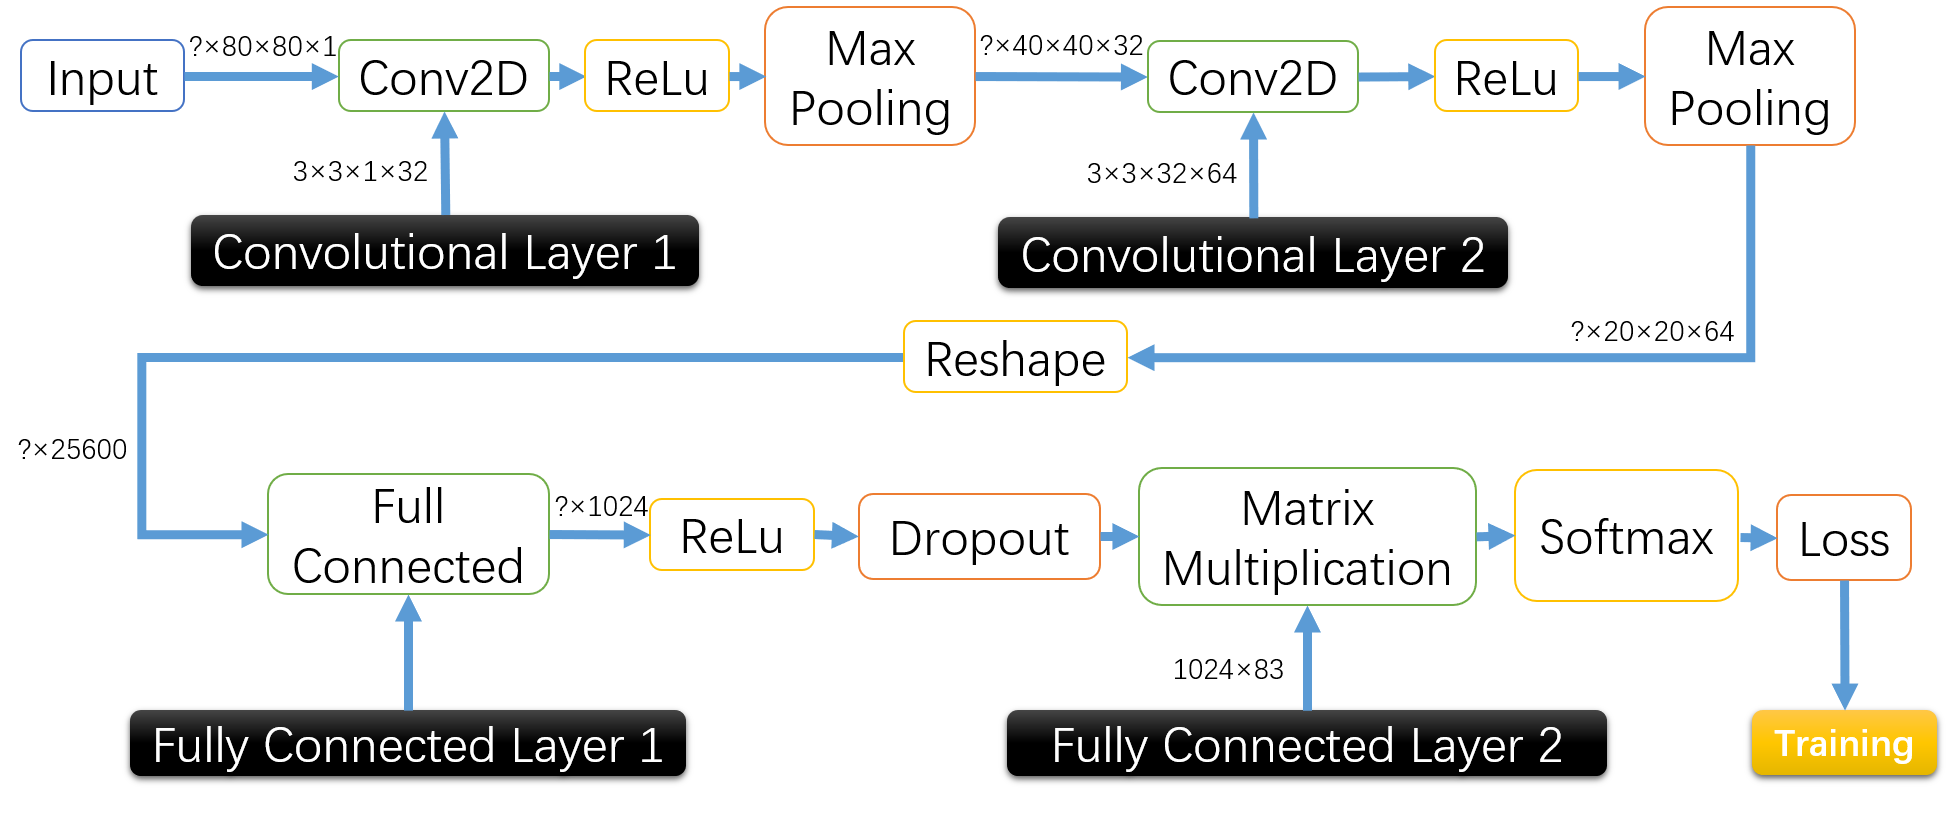
\includegraphics[width=\linewidth]{CNN.png}
	\caption{Structure of convolutional neural networks}
	\label{fig:CNN}
\end{figure}

\begin{itemize}
\item \textbf{Step 1} Load training oracle pictures as a matrix made up of binary numbers, since oracle pictures used here are only monochrome.
\item \textbf{Step 2} Construct a Convolutional Neural Network with two convolutional layers using 3$ \times $3 filters, followed by an activation function ReLU each layer. After that, a 2$ \times $2 max pooling layer whose strike is 2 in a row and 2 in a column at once shrinks the matrices to 50\%$ \times $50\%.
\item \textbf{Step 3} Use a fully connected layer to map the matrices to 1024 nodes. Then, use ReLU as the activation function since Professor Krizhevsky found that\cite{Krizhevsky:2012:ICD:2999134.2999257} ReLU, a nonlinearity activation function is several times faster than hyperbolic tangent $ \tanh $. And then drop out 60\% nodes in case overfitting happens. Without dropout, the model can only predict the word which has been trained. According to \cite{Srivastava:2014:DSW:2627435.2670313}, ``the key idea of dropout is to randomly drop units. Dropout prevents units from co-adapting too much.'' After that, map the 1024 nodes to 83 nodes in the second layer which related the input to one character each and the activation function is softmax.
\item \textbf{Step 4} Test cases are put into the neural network to test the accuracy of the network. The neural network reduces the loss and updates the weights and biases in the network.
\end{itemize}

\subsubsection{Results Visualization, Comparison and Parameter Adjusting}
In the project, we changed one variable at a time and compared its testing accuracy and training speed with the first experiment to find out a better group of parameters. TensorBoard is used to record the performance of each pair of parameters. The parameters which were tested are shown as followed:
\begin{enumerate}
	\item Input size
	\item Convolutional Layer number
	\item Drop out parameter
	\item Learning rate
	\item Filter size
\end{enumerate}
The criteria used to measure the performance of those parameters are two: test accuracy and consumed time.

\subsubsection{Result Analysis and Comparison}
Figure \ref{fig:accuracy} shows the results of seven experiments above and summaries the facts below.
\begin{figure}[h]
	\centering
	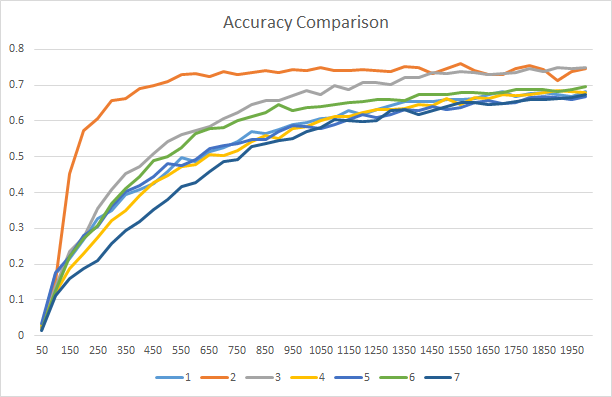
\includegraphics[width=\linewidth]{CNN_Accuracy.png}
	\caption{Test accuracy of 7 experiments}
	\label{fig:accuracy}
\end{figure}
\begin{enumerate}
	\item \textbf{Learning rate in Experiment 1 and 2} When the learning rate was raised from 0.0001 to 0.0005, the consumed time decreased greatly, and the accuracy has been increased. But it is a pity that it is found quite late, so the remaining experiments are conducted using 0.0001 as the learning rate. Using 0.0005 as learning rate can maintain the accuracy at the end, and it also accelerate the training process.
	\item \textbf{Convolutional Layer number in Experiment 1 and 3} Change the convolutional layer from 2 to 3 greatly enhanced the accuracy of the network by 10\% in the end, though the consumed time is increased as well. So it suggests that the deeper neural network (3 layers) has, the better accuracy is achieved when testing.
	\item \textbf{Dropout parameters in Experiment 1, 4 and 5} Dropout is used to prevent the network from overfitting. It drops out some nodes from the first fully connected layer to predict some unknown output using untrained input. Paper \cite{Krizhevsky:2012:ICD:2999134.2999257} mentioned that when using 0.5 as dropout rate, learning can have better performance: ``The neurons which are ``dropped out'' in this way do not contribute to the forward pass and do not participate in backpropagation.'' But in this neural network, the difference of performance does not very obvious with dropout rate varying from 0.5 to 0.6.
	\item \textbf{Filter size in Experiment 1 and 6} The filter size means the view of a computer when scanning the numbers of features in a neural network. A bigger filter size indicates that the machine can ``see'' and catches a bigger feature.
	\item \text{Input size in Experiment 1 and 7} Original Oracle pictures from the website are adjusted without shape transformation. Two versions of the picture adjusting scripts change the size from 80px$ \times $80px to 100px$ \times $100px. The time consumed when a single picture is 100px$ \times $100px increased by 18.83\%, while the accuracy even decreased a little bit. It suggests that there is no need to increase the size of pictures from 80px$ \times $80px pixels to 100px$ \times $100px.
\end{enumerate}

\section{Conditional Generative Adversarial Networks}
Before we actually apply conditional GAN, we have to create a unique dataset for it. After doing statistics for both bronze and oracle bone script dataset, we found that 666 individual characters (recorded in \texttt{Unique\_Characters.txt} file) co-appear in both datasets and each one contains at least one and up to hundreds of different images. For each character, we chose one image to represent it in our paired dataset randomly and two folder with exactly 666 files were created. And then we run the script \texttt{Tools/process.py} to generate image pairs for CGAN training.
\begin{lstlisting}[language = bash, caption = Image Pair Generation]
python3 Tools/process.py \
--input_dir ORACLE \
--b_dir BRONZE \
--operation combine \
--output_dir OUTPUT
\end{lstlisting}
\begin{figure}[h]
	\centering
	
\includegraphics[width=\linewidth]{CGAN_Training_W.png}
	\caption{Samples from Initial Failure}
	\label{fig:failure}
\end{figure}
And then we divided them into training set and validation test with threshold 80\% respectively, which means that there are 532 samples in training set and correspondingly there are 134 ones in validation set (partly showed in Figure \ref{fig:failure}). After several experiments with relatively small epochs (less than 20), we found unfortunately that it did not work because all generated images were purely white, which indicates that in order to create real enough photos, generators learn from input images whose most part is white background. So we had to do some refinements for images to avoid this issues. And the most intuitive approach coming to our mind after a brief brainstorm is to change background of each image.
\begin{figure}[h]
	\centering
	
\includegraphics{Noise.png}
	\caption{Samples from 6 different noise distributions (10px$ \times $10px) (first row from left to right: Gaussian, Impulse and Laplacian; second row from left to right: Multiplicative, Poisson and Random)}
	\label{fig:noise}
\end{figure}
And after checking all possible random images from Figure \ref{fig:noise}, we realised that the simplest ``Random'' distribution may be the most useful in our case. And to avoid letting noise pixels appear on actual monochrome characters, we made the background of character image transparent and merged it to a new noise-processed background (which is showed in Figure \ref{fig:CGAN_training}).
\begin{figure}[h]
	\centering
	
\includegraphics[width=\linewidth]{CGAN_Training_R.png}
	\caption{Samples from CGAN training dataset}
	\label{fig:CGAN_training}
\end{figure}

We started our training with batch size = 32, learning rate = 0.0002 and maximum epoch = 200. Part of results can be seen in Appendix \ref{ch:appendix_2} and more validation results are available on our GitHub repository. Obviously, current results are not ideal, so we continued to train our CGAN models with much more epochs (5000 and 20000, which are listed in Appendix \ref{ch:appendix_3} and \ref{ch:appendix_4} separately.

Eventually, according to GAN Zoo\footnote{\url{https://github.com/hindupuravinash/the-gan-zoo}}, there are hundreds of different GANs available. We also went through some of them and found potential ones to be our next candidates.
	\chapter{Tuning \& Optimisation}
After we build a basic structure of our project, we noticed that several issues can be refined and improved.

\section{Mathematical Morphology}\label{sec:MM}
We use mathematical morphology to reduce efficiently calculation by increasing the number of 0s in image matrix and keeping original character structures to maximum extent simultaneously. And images loaded from disk can be compressed into sparse matrices, whose functionality is provided by \texttt{scipy.sparse}, and later TensorFlow \texttt{SparseTensor} is applied to speed up calculation and save disk space.

MM is originally applied on binary images, and fortunately all crawled grayscale .gif images with only two colormap entries (pure white \#FFFFFF and pure black \#000000). According to ImageMagick user manual, ``the larger the kernel, the longer the morphological methods will take'', and we prefer to use smaller kernel size to fulfil the same task. In order to increase run-time for our CNN models, we want to keep effective and simplified information in our training images and do not lose topological structures, thereby thinning algorithm in digital image processing coming to our mind. It is a type of topological skeleton, but computed by means of morphological openings. According to Lantu\'{e}joul\cite{serra1983image}, the formula to getting the skeleton of a binary image $ X \subset \mathbb{R}^2 $:
\[ S(X) = \displaystyle \bigcup_{\rho > 0}\bigcap_{\mu > 0}[(X\ominus \rho B)-(X\ominus \rho B)\circ\mu\bar{B}] \]
where $ \ominus $ and $ \circ $ are erosion and opening as we mentioned before, $ \rho $ is the radius and $ \bar{B} $ is the closing result of $ B $ itself. And here $ \rho $ is the size of our structuring element as a matter of fact. And fortunately, we can implement this algorithm by built-in OpenCV functions easily (of course, a little differently).
\begin{lstlisting}[language = Python, caption = Skeletonisation]
img = cv2.imread(FILE_NAME,0)
rho = 3 # Radius.
size = np.size(img)
element = cv2.getStructuringElement(cv2.MORPH_CROSS, (rho, rho))
done = False
while ( not done ):
	eroded = cv2.erode(img, element)
	temp = cv2.dilate(eroded, element)
	temp = cv2.subtract(img, temp)
	skel = cv2.bitwise_or(skel, temp)
	# `skel` will contain skeletonised images.
	img = eroded.copy()
	zeros = size - cv2.countNonZero(img)
	if zeros == size:
		done = True
\end{lstlisting}
And sample of images can be seen below :
\begin{figure}[h]
	\centering
	
\includegraphics{80x80.png}
	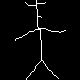
\includegraphics{80x80_thinning.png} 
	\caption{ Comparison of original image (left) and skeletonised one (right)}
\end{figure}
After small scale tests, newly-generated dataset speed up the training process, reducing one third of run-time.

\section{TensorFlow-related Tuning}
\subsection{Data Type}
The default data type (\texttt{tf.DType}) for numbers in tensors is \texttt{tf.float32} and for better memory performance, we decided to change it into \texttt{tf.bfloat16}, 16-bit truncated floating-point type, which makes both our neural network models even fit on mid-end computers with 7.7 GiB main memory with 1000 MiB swap, without affecting accuracy obviously (less than 1\% dropping rate).

\subsection{TFRecord}
Unlike other high-level deep learning API such as Keras\footnote{\url{https://keras.io/}}, TensorFlow does not implement HDF5 interface, a high-performance portable structured data format developed by HDF Group\footnote{\url{https://www.hdfgroup.org/}}, or supports it via h5py\footnote{\url{https://www.h5py.org/}}, though the possible alternative (tftables\footnote{\url{https://github.com/ghcollin/tftables}}) is available without official support. Instead, TensorFlow created its own pipeline-compatible API \texttt{tf.data} to create high-speed data structure \texttt{TFRecord}, to replace previous hard-to-use interface \texttt{QueueRunner}\cite[pp.~338]{geron2017hands} since 2017. Pre-processing data can be somewhat time-consuming, but once TFRecord files is an one-off solution of efficient training.

There are several ways to prepare data in TensorFlow, and the simplest one is preparing in Python language, using \texttt{tf.placeholder} as variable place holders and being fed into \texttt{feed\_dict} parameter. When in each step of training or testing, new batch of data come into models.

In practice, we try to use \texttt{Numpy} arrays directly. When all data is loaded into memory, dataset can be created by arrays. And after small scale experiments, we found that the method may copy the same block array contents for multiple times, which lessen loading speed in our case.

According to TensorFlow official API manual\footnote{\url{https://www.tensorflow.org/api\_guides/python/reading\_data}}, \texttt{feed\_dict} is the least efficient way to load data.
In TensorFlow, every independent data is regarded as an object in \texttt{tf.train.Example}, using \texttt{proto3} protocol to serialise data.
Here is the code snippet to create a TFRecord file by reading image contents and setting a unique label.
\begin{lstlisting}[language = Python, caption = TFRecord File Creation]
with open(FILENAME, "rb") as fp:
	image_data = fp.read()
	features = {
	"Images": _bytes_feature(image_data),
	"Labels": _int64_feature(label_index),
	}
	example = tf.train.Example(features =\
tf.train.Features(feature = features))
	tfrecord_writer.write(example.SerializeToString())
\end{lstlisting}
Where \texttt{\_bytes\_feature} and \texttt{\_int64\_feature} is helper functions to create a \texttt{Feature} object in TensorFlow.
And these data can be loaded into TensorFlow by simply \texttt{dataset = tf.data.TFRecordDataset(FILENAME)} and according to pipeline mechanism, speed improvement is dramatic. (In our case, data loading time is reduced from more than 50 seconds to 20 seconds.)

\subsection{Eager Execution}
Google TensorFlow development team released eager evaluation as experimental feature in 2017 and became formal after TensorFlow v1.7.0, which is ``an imperative, define-by-run interface'' to achieve faster debugging process more interactively and intuitively. Without building graphs as usual, basically it turns TensorFlow from declarative language to imperative one. Although we write this report, not all APIs support eager evaluation currently.

For most cases, user simply invoke \texttt{tf.enable\_eager\_execution()} at the beginning of TensorFlow-related code. And noticeably, eager evaluation works pretty good with \texttt{Numpy}. Although there are only a small of EE-specific APIs, most of current APIs are EE-compatible.
\begin{lstlisting}[language = Python, caption = Rewritten CNN Core Code Using Eager Eexecution]
EPOCHES = 1000
optimizer = tf.train.AdamOptimizer(learning_rate = 1e-3)
batch_size = 32
for step in range(EPOCHES):
	batch_data, batch_label = raw_data.train.next_batch(batch_size)
	batch_data = batch_data.reshape([-1 ,48, 48, 1])
	optimizer.minimize(lambda: loss(step, batch_data, batch_label))
\end{lstlisting}

\section{General Hyperparameter Adjustments}
In machine learning, a hyperparameter is a parameter whose value is set before the learning process begins. And there are some tricks that we learnt from other ones' code when we train our GANs, which may not be verified by traditional mathematical methods. However, in practice they work very well and we try to find evidences to back them.
\begin{itemize}
	\item According to \cite{Srivastava:2014:DSW:2627435.2670313}, we set our dropout rate to 50\%.
	\item ADAM optimiser is always our priority based on \cite{DBLP:journals/corr/SalimansGZCRC16}.
	\item At least in our CycleGAN training, we sometimes found that if we train discriminator more frequently, we can get a better result.
	\item Apply $ \tanh $ on the output of the last layer of the generator $ G $.
	\item In GAN-related papers, the loss function used to optimise $ G $ is always $ \min(\log{(1-D)}) $, but after reading several open-source code, people tend to use $ \max(\log{D}) $ practically. It is said that ``the first formulation has vanishing gradients early on''\cite{goodfellow2014generative}.
	\item After multiple experiments, we noticed that general performance of sampling from uniform distribution is much worse than sampling from Gaussian distribution. And the paper\cite{DBLP:journals/corr/White16a} seems to support our ideas in details.
	\item For Conditional GANs, use an embedding layer, and keep embedding dimensionality low and upsample to match image channel size.
	\item Also some suggests that label smoothing may be a good option to fast converge. Instead of giving a defined integer value (fake = 0 and real = 1), one can give a float-point number from 0.0 to 0.5 to stand for fake label and a number from 0.5 to 1.0 to stand for real one.  But in reality, we cannot apply that since it is really difficult to change code from \texttt{int32}-represented labels to \texttt{float32}-represented ones without any mistakes.
\end{itemize}
	\chapter{Conclusion}
In conclusion, we collected more than 100 thousand ancient Chinese character images, processed them in a suitable and well-considered fashion. Then we applied CNN on recognition tasks and achieved relatively acceptable results compared to traditional ones. Eventually GAN, a neural network technique with data generation feature, gave us feedbacks of Bronze-script-like / modern-Chinese-character-like images by inputting oracle bone script characters into our programs.
	\chapter{Possible Future Work}
Here are several work that may be done in the future and possible development directions:
\begin{itemize}
	\item First Visualise first-layer weights to decide next training direction; visualise convolutional kernels of CNN using Deep Visualization Toolbox\footnote{\url{https://github.com/yosinski/deep-visualization-toolbox}} and try to gain more insight into the functionality of each layer, improving accuracy further.
	\item Continue applying skeleton recognition skills on our trained model.
	\item DualGAN\cite{DBLP:journals/corr/YiZTG17}, which is an enhanced version of CGAN, can be applied to improve performance;and DiscoGAN\cite{DBLP:journals/corr/KimCKLK17} also uses two pairs of generators and discriminators like CycleGAN, but in DiscoGAN, authors used conv, deconv and leaky ReLU function to build generators and used only conv along with ReLU to make discriminators, which may have bright future on character recognition.
	\item For simplifying our code, and eliminating boilerplate code, we may turn lightweight but experimental framework TensorFlow-Slim\footnote{\url{https://github.com/tensorflow/tensorflow/tree/master/tensorflow/contrib/slim}}, which can at least increase readability and maintainability in our small-scale experiments. Or some APIs offering higher-level logic and abstraction is also a nice potential option, including TFLearn\footnote{\url{http://tflearn.org/}} and Theano (mentioned in \ref{ch:setup}) instead of sticking on TensorFLow.
	\item Examine potential relationships between oracle bone scripts and other Chinese scripts.
	\item Extract inscriptions directly from stone rubbing photos. And word embedding can be applied since context is available. Here is websites that could be used as data sources:
	\begin{itemize}
		\item \url{http://www.guoxuedashi.com/} (in simplified Chinese) contains a huge amount of high definition photocopies of classic ancient Chinese collections.
		\item \url{http://sinology.teldap.tw/index.php/reslook/rs144/rs14411} (in traditional Chinese) is set up by Academia Sinica and heavily relies on unearthed literature of oracle bone scripts.
		\item \url{http://sinology.teldap.tw/index.php/reslook/rs144/rs1442} is similar to the one above but based on bronze scripts.
	\end{itemize}
\end{itemize}
	\addToTOC{References}
	%\makeBibliographyPage
	\bibliographystyle{IEEEtran}
	\bibliography{References/references}

	%\makeAppendixPage
	\appendix
	\chapter{Currently Unused Data}
\label{ch:appendix_1}
There are some data that we collected but did not use for some reasons. Anyone who is interested can find them in our project GitHub repository (in \texttt{Data/Unused} directory); meanwhile, there are some useful websites that we found during this tise without using frequently and we hope that the public sharing can reduce time for gathering information if someone will conduct similar researches like what we did. Therefore we list them below:
\begin{itemize}
	\item More than 60000 processed seal script character images from Liu Shu Tong and Shuowen Jiezi are packed along with oracle bone script and bronze script data that we used in .zip format; ancient Chinese font files in .ttf format from various sources. Details can be found in \texttt{README.txt} file.
	\item Two formal proposals from Taipei Computer Association	(TCA) and China on tentative allocation of Plane 3, the TIP (Tertiary Ideographic Plane) including distinct 10982 small seal scripts (divided into 14 volumes) and 1463 oracle bone scripts to be standardised.
	\item \url{http://humanum.arts.cuhk.edu.hk/Lexis/lexi-mf/} is called Multi-function Chinese Character Database, maintained by The Chinese University of Hong Kong. It provides a structured display for each character; also a special function of English-Chinese lookup is offered. It is language-friendly for Mandarin, English and even Cantonese dialect users.
	\item \url{http://xiaoxue.iis.sinica.edu.tw/} (in traditional Chinese) is a Chinese character database built by Institute of Information Science, Academia Sinica; it claims that it collects more than 200 thousand glyphs from diverse sources.
\end{itemize}
	\chapter{200-epoch CGAN Results}\label{ch:appendix_2}
Here is an HD version of image samples from CGAN training after 200 epochs, converting oracle bone script characters into corresponding bronzes-script-like characters.
\begin{figure}[h]
	\centering
	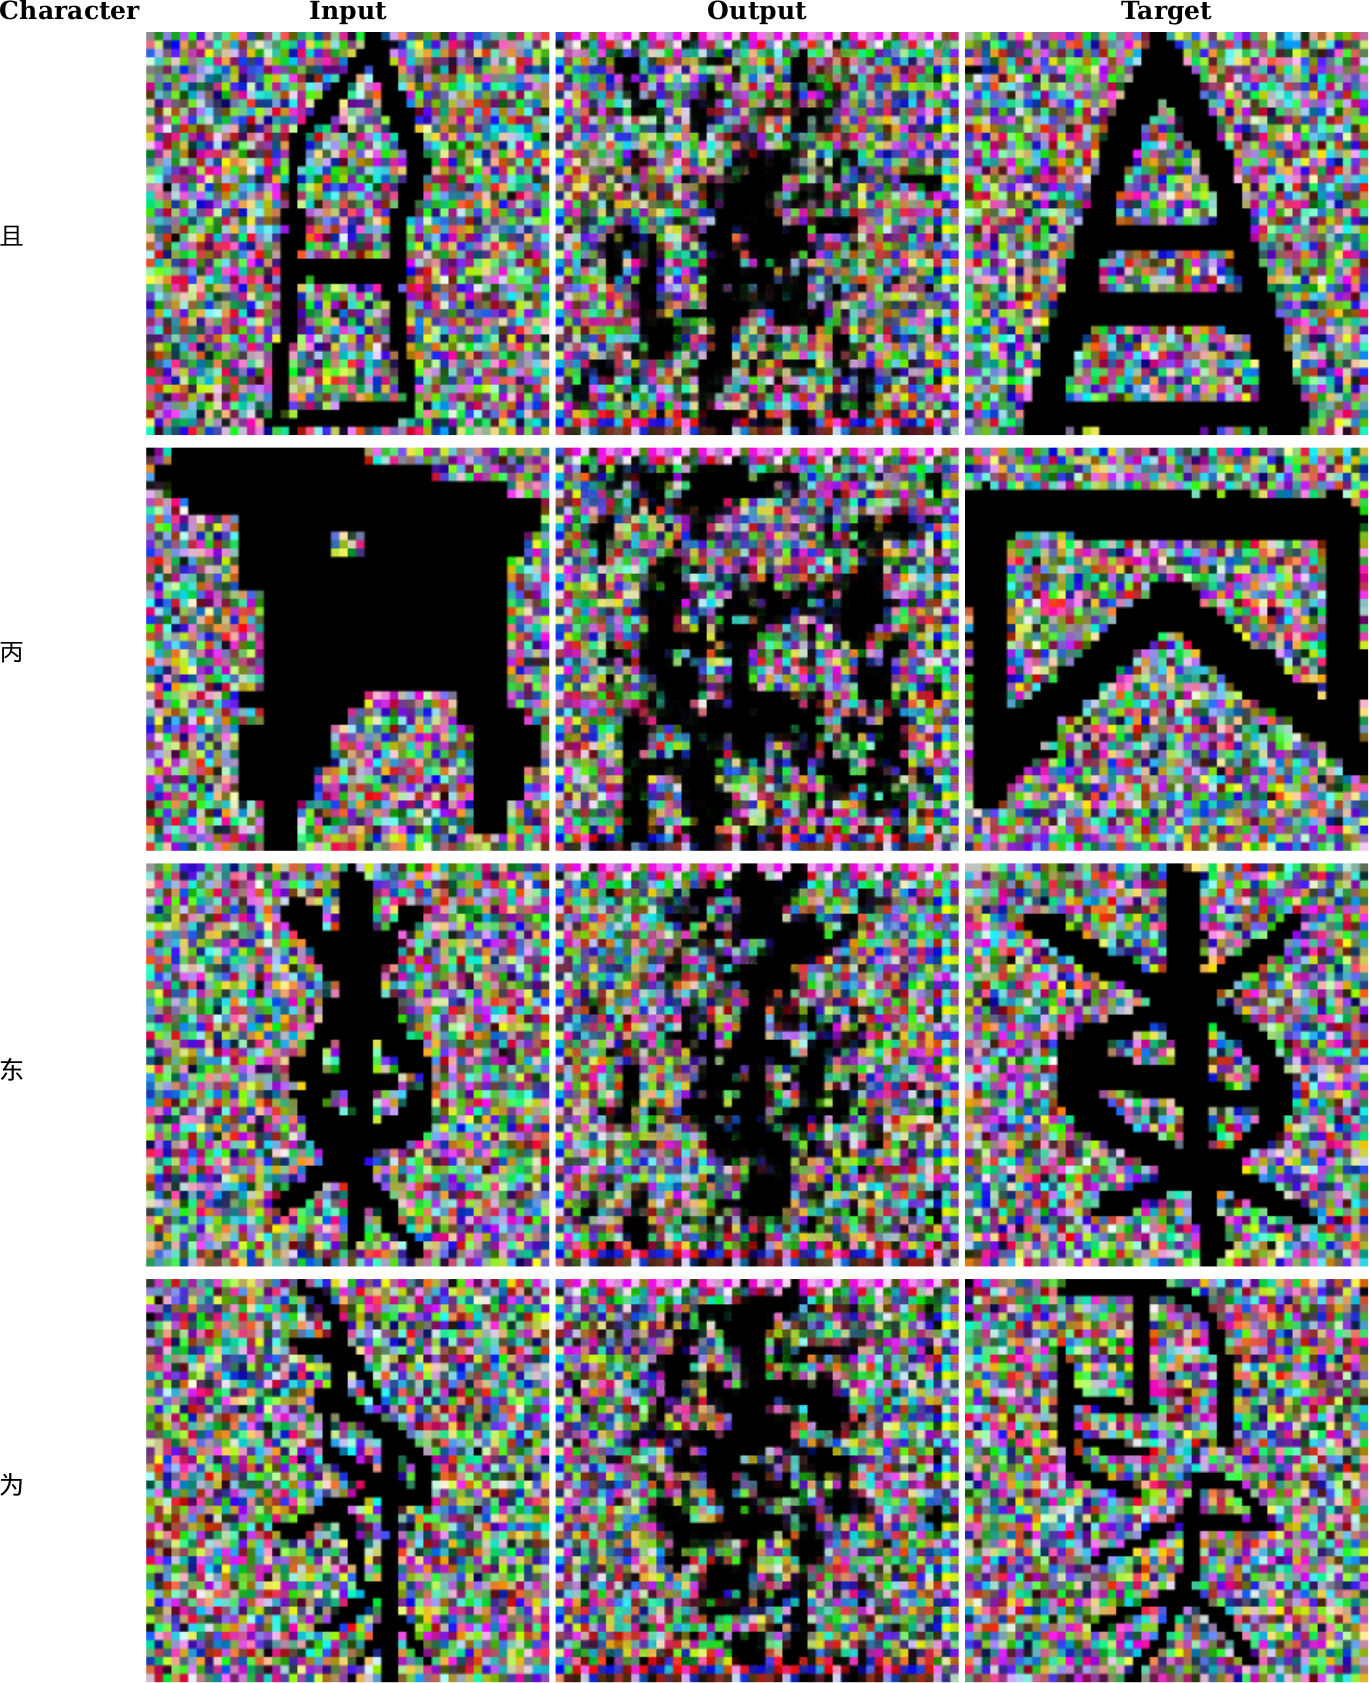
\includegraphics[scale=0.65]{O2B_200.png}
	\caption{\label{fig:O2B_200} Samples after 200 Epochs}
\end{figure}
	\chapter{5000-epoch CGAN Results}\label{ch:appendix_3}
Here is an HD version of image samples from CGAN training after 5000 epochs, converting oracle bone script characters into corresponding bronze-script-like characters.
\begin{figure}[h]
	\centering
	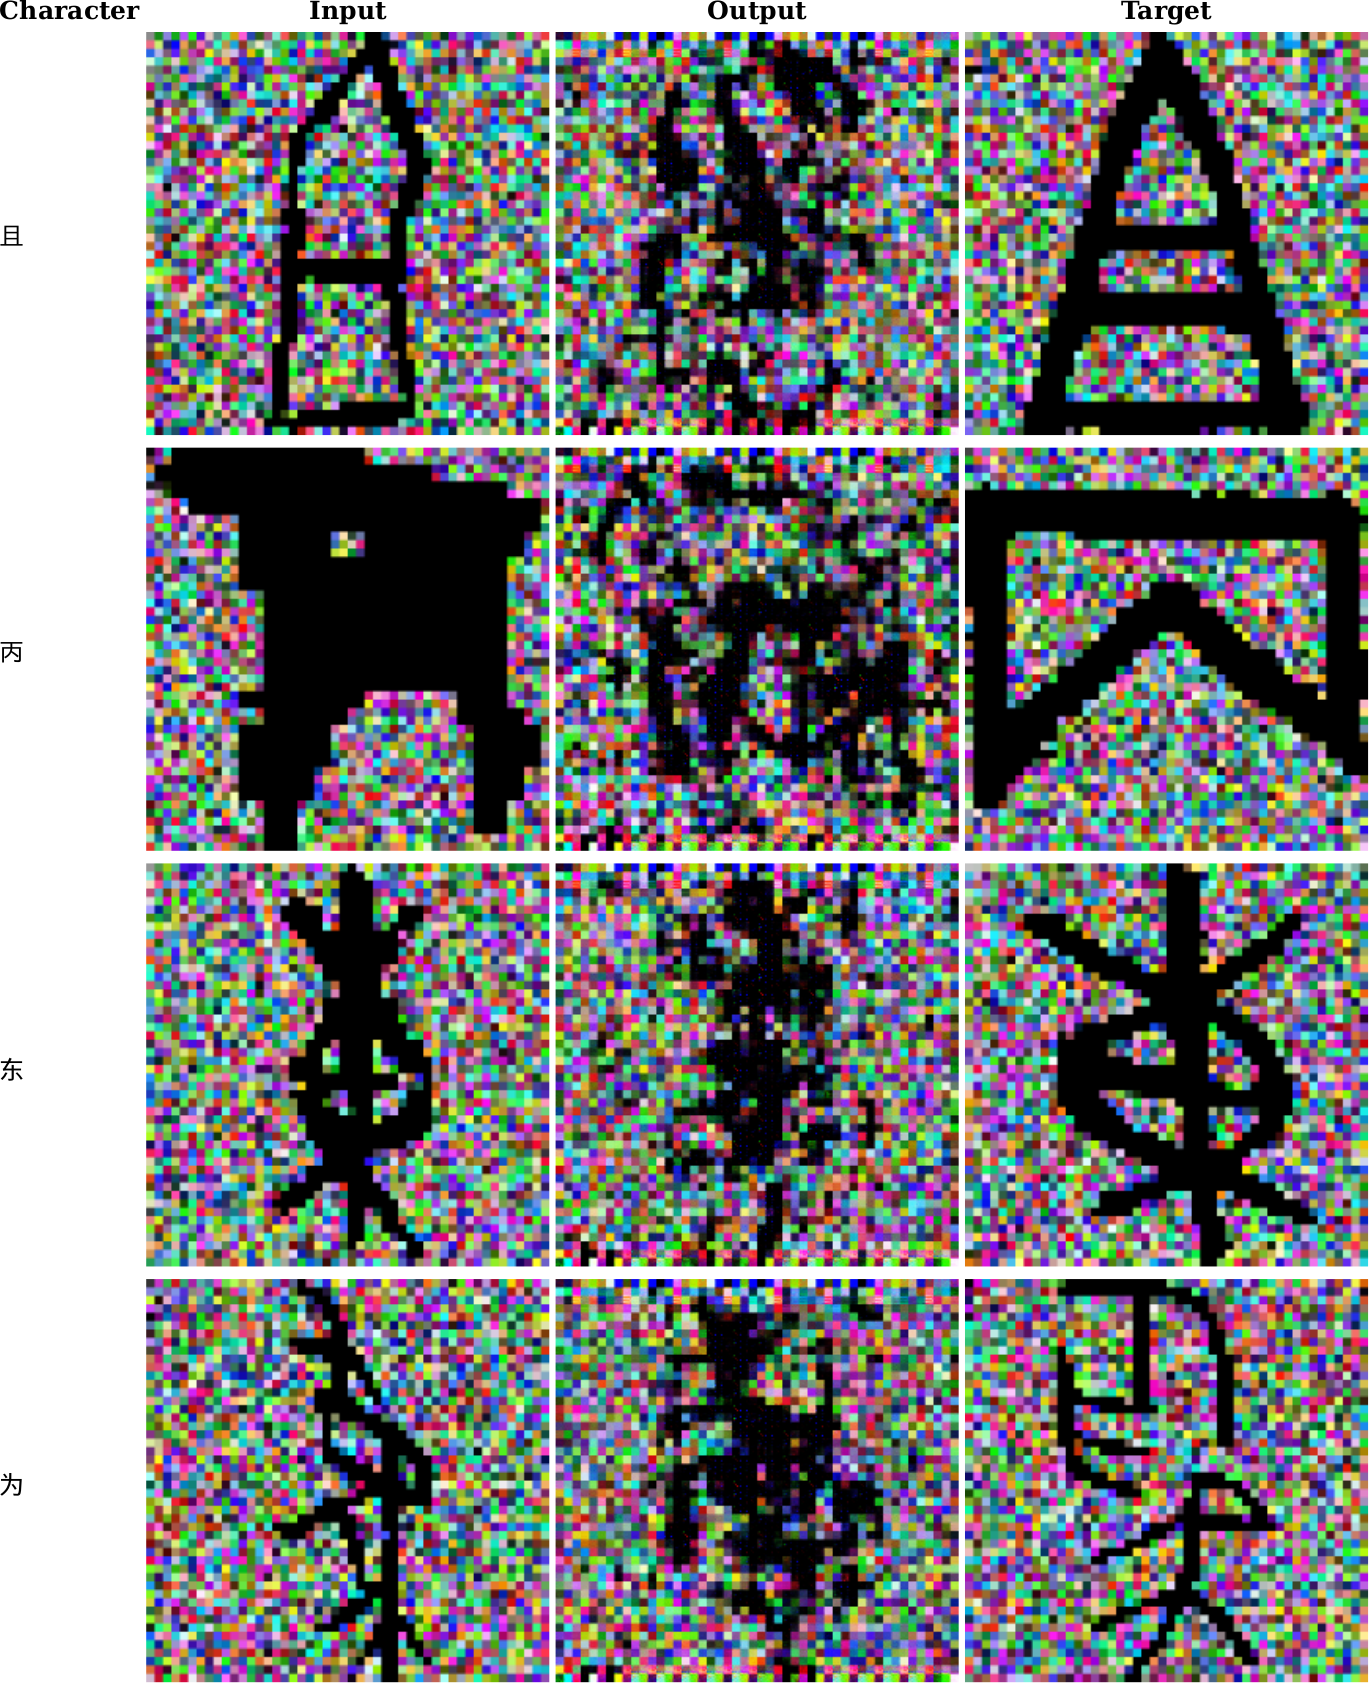
\includegraphics[scale=0.65]{O2B_5000.png}
	\caption{\label{fig:O2B_5000} Samples after 5000 Epochs}
\end{figure}
	\chapter{20000-epoch CGAN Results}\label{ch:appendix_4}
Here is an HD version of image samples from CGAN training after 20000 epochs, converting oracle bone script characters into corresponding bronze-script-like characters.
\begin{figure}[h]
	\centering
	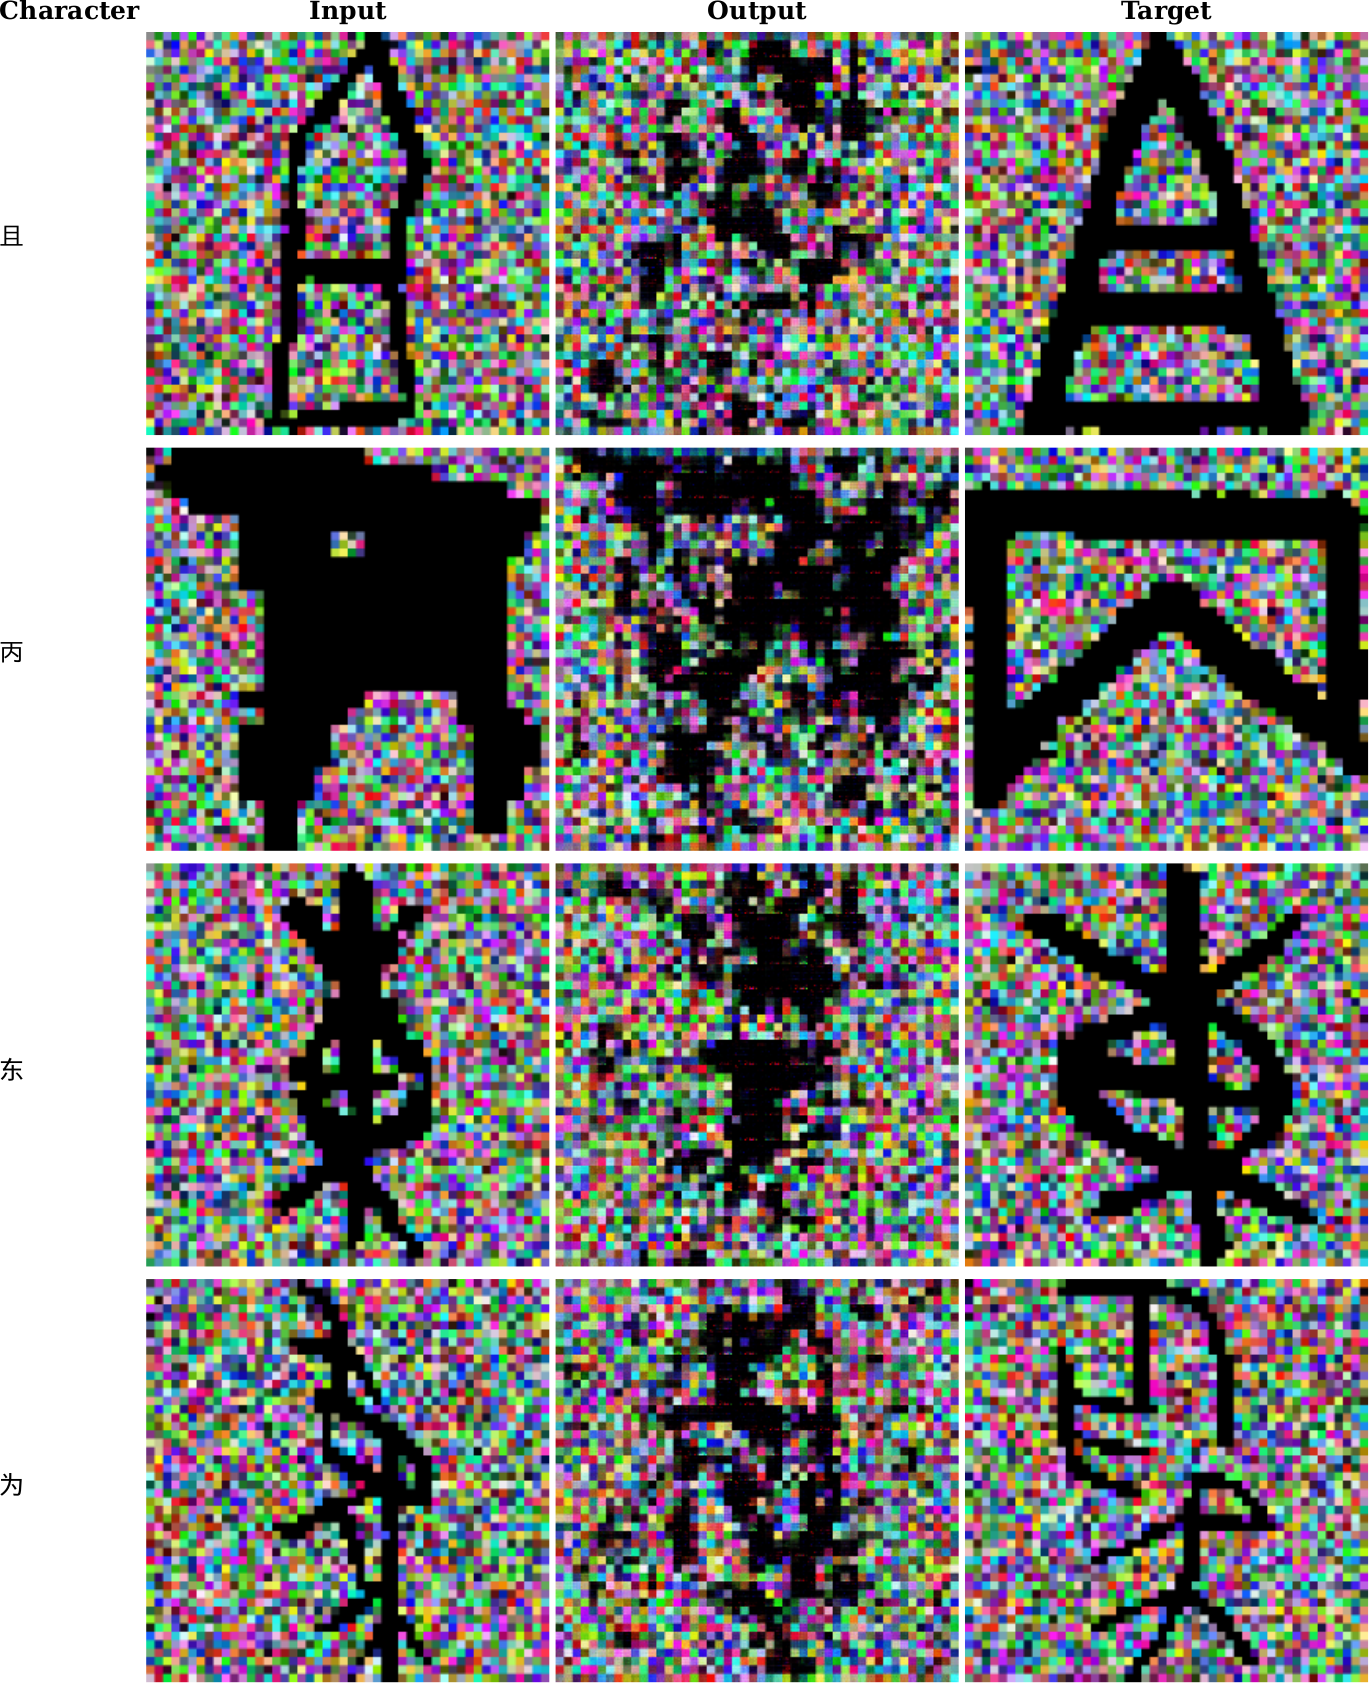
\includegraphics[scale=0.65]{O2B_20000.png}
	\caption{\label{fig:O2B_20000} Samples after 20000 Epochs}
\end{figure}
	\chapter{10000-epoch CGAN Results with Reverse Conversion}\label{ch:appendix_5}
Here is an HD version of image samples from CGAN training after 20000 epochs, converting bronze script characters into corresponding oracle-bone-script-like characters.
\begin{figure}[h]
	\centering
	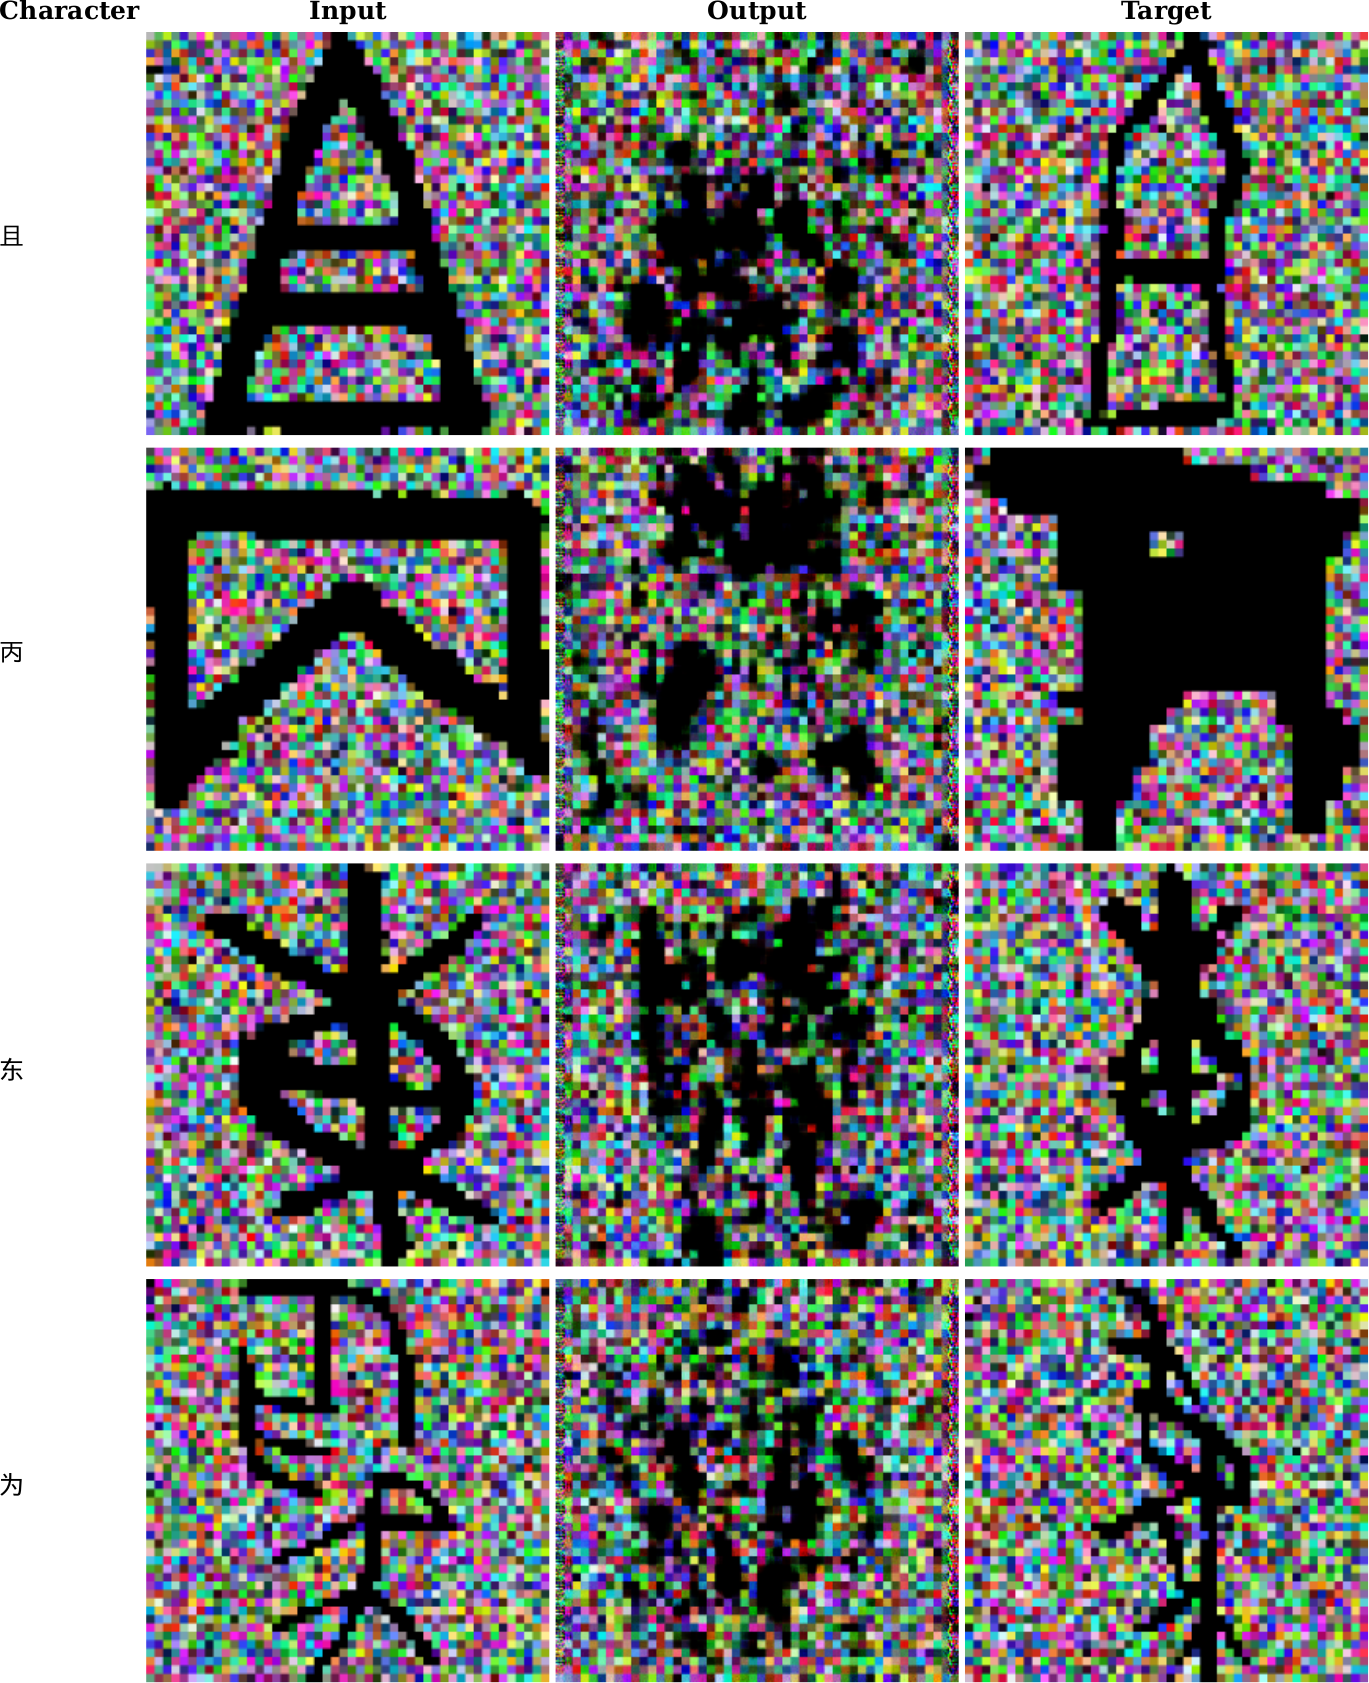
\includegraphics[scale=0.65]{B2O_10000.png}
	\caption{\label{fig:B2O_10000} Samples after 10000 Epochs with Reverse Conversion}
\end{figure}
	\nocite{*}
\end{document}